
\section{Conceptual Architecture}
\label{sec:architecture}

\subsection{Box-and-Arrow Diagram}
\label{sec:box-and-arrow-diagram}

The top-level subsystems are the GUI Front End, Multiplexer, Mux Client, Mux Server, SSH Client, and Configuration Engine, with the Terminal Emulation Core and PTY completing the remote-side path. The diagram separates the Mux Client and Mux Server because they occupy different hosts and have distinct responsibilities. Configuration Engine is drawn as a dashed box with dashed arrows, since it supplies settings to the GUI Front End and Multiplexer at startup and on hot-reload rather than participating in the per-request control and data flow the solid arrows depict. The diagram also shows the external SSH Server and Shell.
\begin{figure}[H]
 \centering
 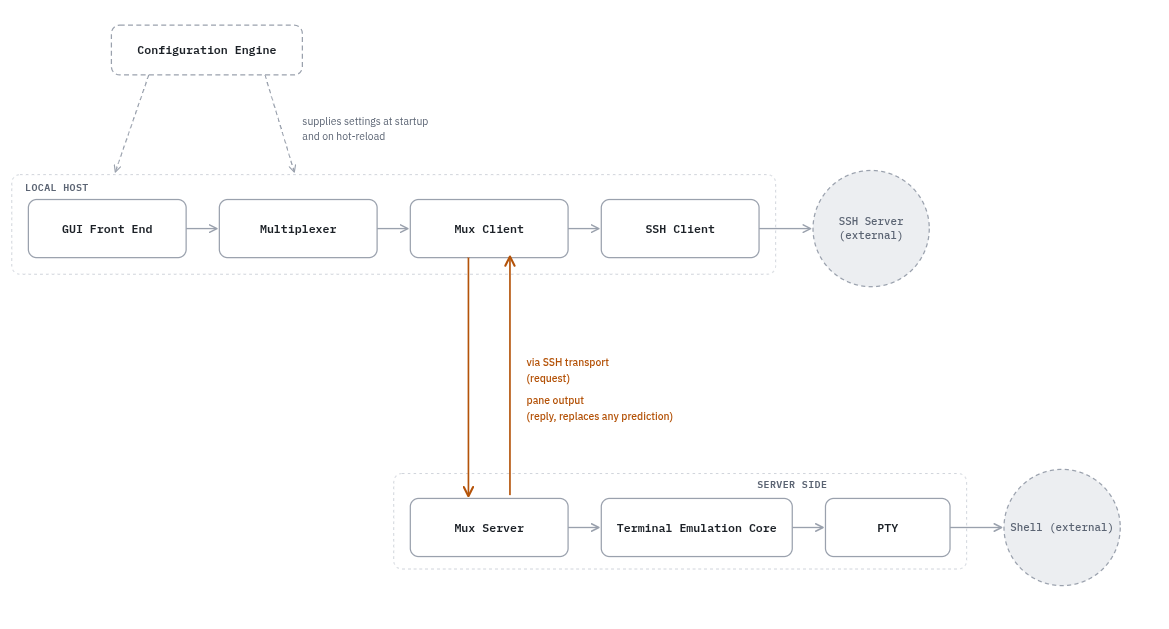
\includegraphics[width=\linewidth]{prism-uploads/image_9.png}
 \caption{Box-and-arrow diagram derived from the sequence diagrams, plus the Configuration Engine (dashed)}
 \label{fig:derived-box-and-arrow}
\end{figure}

\paragraph{Legend.} Solid arrows indicate a dependency: the source depends on the target. The labeled arrow shows the main data flow. Grey dashed shapes represent components external to WezTerm and not part of its codebase.


\subsection{Subsystems and Their Responsibilities}
\label{sec:subsystems}

WezTerm’s architecture utilizes a distributed, modular approach that separates local rendering from remote state management. To support remote sessions, the architecture divides responsibilities between local routing components, network transports, and remote authoritative servers. The internal design relies on isolated Rust crates to enforce these boundaries.

\textbf{1. GUI Front End}

The GUI Front End manages the physical windowing system and visual rendering on the local host. It captures user inputs, such as key presses, and repaints changed lines or local panes on the physical display. Internally, this subsystem utilizes a dedicated windowing abstraction crate to interface with OS-specific APIs (e.g., Wayland, X11, Cocoa, or Direct2D), ensuring the core event loop remains platform-agnostic. For rendering, it employs a two-stage pipeline. First, a font shaping engine utilizes libraries like HarfBuzz and FreeType to calculate precise glyph placements for ligatures, complex scripts, and fallback fonts (such as Color Emojis). Second, these rasterized glyphs are cached into a texture atlas. The GUI Front End then issues draw calls to a graphics API (WebGPU or OpenGL) to composite this atlas onto the screen \cite{gui-crate}. It acts as a pure presentation layer and defers all state management and event routing to the Multiplexer.

\textbf{2. Multiplexer}

Operating on the local host, the Multiplexer acts as the local routing layer and state orchestrator. It receives domain attachment requests and key events from the GUI Front End. The Multiplexer relies on a strict hierarchical data model to manage logical state: Workspaces contain Windows, Windows contain Tabs, and Tabs contain Panes \cite{mux-crate}. It holds the authoritative state for all local panes and acts as the router for remote panes, forwarding remote interactions directly to the Mux Client.

\textbf{3. Mux Client}

The Mux Client serves as the local proxy for remote domains. It initiates the attachment process by opening a session through the SSH Client. Once authenticated, it retrieves the remote windows, tabs, and panes via RPC (Remote Procedure Call) serialization and adds them as client panes locally. During active sessions, the Mux Client forwards key events over the SSH channel. To mitigate network latency, it maintains a predictive control loop: if the network delay exceeds a configured threshold, the Mux Client immediately generates a predicted echo of the keystroke and notifies the Multiplexer to render it. When the actual pane output arrives from the remote server, it overwrites the predicted text. The Mux Client also handles local teardown, dropping a domain's panes locally upon a user detach command or a lost network connection.

\textbf{4. SSH Client}

The SSH Client handles network protocol integration on the local host. Instead of relying on external system binaries, it utilizes a native Rust SSH implementation to securely transport multiplexer RPCs \cite{ssh-crate}. It resolves host settings, verifies unknown host keys, and authenticates connections to an external SSH Server on the target machine.

\textbf{5. Mux Server}

The Mux Server is the authoritative backend daemon running on the remote host, typically joining a Unix socket. Its primary responsibility is maintaining the continuous lifecycle and logical state of remote panes, tabs, and windows. It receives key event bytes over the SSH channel and writes those exact byte streams directly to the PTY. Conversely, it listens for screen changed events triggered by the Terminal Emulation Core. To optimize network bandwidth, the Mux Server computes the delta of the screen matrix and pushes only the changed lines back to the Mux Client. Because it stores the entire workspace hierarchy in memory independently of the transport layer, it ensures panes survive network timeouts and client detaches, keeping the underlying PTY running indefinitely until the user explicitly re-attaches or the remote program exits.

\textbf{6. Terminal Emulation Core}

Operating on the remote host alongside the Mux Server, this core logic engine acts as a pure virtual terminal state machine. It runs on a dedicated reader thread, parsing raw output bytes from the PTY. It interprets ANSI and ECMA-48 escape sequences to manipulate a mathematical model of the terminal. Internally, this model is a 2D grid array of cell objects. When an escape sequence dictates a visual change, the core mutates the specific cell attributes in the grid and triggers a state update \cite{term-crate}. This grid isolation ensures the core never interfaces with actual pixels.

\textbf{7. PTY (Pseudo-Terminal)}

The PTY acts as the OS-level bridge on the remote host. It provides the file descriptors necessary to spawn and manage external shell processes (such as bash or zsh). It routes input bytes from the Mux Server into the shell's standard input, and feeds shell standard output bytes back to the Terminal Emulation Core. It manages end-of-file states and applies exit behaviors when a remote program terminates, signaling the Mux Server to drop the pane.

\textbf{8. Configuration Engine}

The Configuration Engine is an isolated subsystem that embeds a Lua runtime to evaluate user configuration dynamically. It parses Lua scripts at startup to construct a static configuration struct dictating terminal behavior, keybindings, and UI themes. To support multi-threaded hot-reloading without stalling the GUI Front End, the engine monitors the configuration file using OS-level file watchers on a background thread. Upon detecting a change, it safely hot-swaps the active configuration state across the application via thread-safe atomic references \cite{config-crate}.

\subsection{Dependencies Among Subsystems}
\label{sec:dependencies}

At the foundational layer on the remote host, the Terminal Emulation Core depends directly on the operating system's PTY interfaces to route input and output bytes to and from external shell processes. The Mux Server depends entirely on the Terminal Emulation Core to translate those raw output bytes into an updated logical screen matrix. Crossing the network boundary, the local Mux Client depends heavily on the remote Mux Server to retrieve pane states, list active windows, and synchronize remote actions. This dependency is bridged by the SSH Client, which the Mux Client relies upon to resolve host settings, verify host keys, and establish an authenticated transport layer with an external SSH Server. 

On the local host, the Multiplexer depends on the Mux Client to handle the routing and session management for all remote domains. The GUI Front End sits at the top of the hierarchy, depending exclusively on the Multiplexer to receive pane output notifications, structural updates, and logical state. The GUI Front End cannot function or render meaningful text without the Multiplexer supplying this synchronized state. Additionally, both the GUI Front End and the Multiplexer depend on the Configuration Engine to supply the dynamic runtime parameters parsed from the Lua environment.

\begin{table}[!htbp]
  \centering
  \caption{Dependencies among the subsystems discussed in this report.}
  \label{tab:dependencies}
  \begin{tabularx}{\linewidth}{@{}llX@{}}
    \toprule
    \textbf{From} & \textbf{To} & \textbf{What the dependency represents} \\
    \midrule
    Terminal Emulation Core & OS PTY Interfaces & Route input and output bytes to and from external shell processes. \\
    Mux Server & Terminal Emulation Core & Translate raw output bytes into an updated logical screen matrix. \\
    Mux Client & Mux Server & Retrieve pane states, list active windows, and synchronize remote actions. \\
    Mux Client & SSH Client & Resolve host settings, verify host keys, and establish authenticated transport layer. \\
    Multiplexer & Mux Client & Handle routing and session management for all remote domains. \\
    GUI Front End & Multiplexer & Receive pane output notifications, structural updates, and logical state. \\
    GUI Front End \& Multiplexer & Configuration Engine & Supply dynamic runtime parameters parsed from the Lua environment. \\
    \bottomrule
  \end{tabularx}
\end{table}
